\documentclass[12pt]{report} % add 'draft' to suppress figures
% Double-spaced, single-column format for IEEE journal submission
% \documentclass[12pt,journal,draftclsnofoot,onecolumn]{IEEEtran} 
\usepackage{wrapfig,booktabs,fancyhdr,amsmath,amsfonts,tabularx,numprint}
\usepackage{cite,bm,bbm,amssymb,amsthm,url,multirow,times,enumitem,comment}
\usepackage{mathtools,siunitx,balance,tikz,adjustbox,graphicx,array}
\usepackage[font=footnotesize]{subcaption}
\usepackage[linesnumbered,ruled]{algorithm2e}
\usepackage[colorlinks=true, linkcolor=black, citecolor=blue, urlcolor=blue]{hyperref}
\usepackage{geometry}
 \geometry{
 a4paper,
 total={170mm,257mm},
 left=20mm,
 top=20mm,
 }
 \usepackage[acronym,nomain,nonumberlist]{glossaries}
 \makeglossaries
 \usepackage{mdframed}

 \newcommand{\vb}{\boldsymbol}
\newcommand{\vbh}[1]{\hat{\boldsymbol{#1}}}
\newcommand{\vbc}[1]{\check{\boldsymbol{#1}}}
\newcommand{\vbb}[1]{\bar{\boldsymbol{#1}}}
\newcommand{\vbt}[1]{\tilde{\boldsymbol{#1}}}
\newcommand{\vbs}[1]{{\boldsymbol{#1}}^*}
\newcommand{\vbd}[1]{\dot{{\boldsymbol{#1}}}}
\newcommand{\abs}[1]{\left|{#1}\right|}
\newcommand{\by}{\times}
\newcommand{\tr}{\mathsf{T}}
\newcommand{\sfrac}[2]{\textstyle \frac{#1}{#2}}
\newcommand{\ba}{\begin{array}}
\newcommand{\ea}{\end{array}}
\newcommand{\sinc}{\text{sinc}}
\newcommand{\define}{\triangleq}
%\newcommand{\define}{\coloneqq}
\newcommand{\cnr}{C/N_0}
\newcommand{\sgn}{\text{sgn}}
\renewcommand{\Re}{\mathbb{R}}
\renewcommand{\Im}{\mathbb{I}}
\newcommand{\E}[1]{\mathbb{E}\left[ #1 \right]}
\newcommand{\brm}[1]{\bm{\text{#1}}}
\newcommand{\round}[1]{\ensuremath{\lfloor#1\rceil}}
\DeclareMathAlphabet{\mathpzc}{OT1}{pzc}{m}{it}
\DeclareMathOperator*{\argmin}{\arg\!\min}
\DeclareMathOperator*{\argmax}{\arg\!\max}

% Macros for this paper
\newcommand{\Fc}[1]{\ensuremath{F_{\text{c}#1}}}
\newcommand{\Fs}{\ensuremath{F_\text{s}}}
\newcommand{\Fsr}{\ensuremath{F_\text{sr}}}

\newacronym{PL}{PL}{Path loss}
\newacronym{LOS}{LOS}{Line of sight}
\newacronym{NLOS}{NLOS}{Non-line of sight}
\newacronym{BW}{BW}{Bandwidth}
\newacronym{iid}{i.i.d.}{independent and identically-distributed}
\newacronym{CLT}{CLT}{Central Limit Theorem}
\newacronym{GRV}{GRV}{Gaussian random variable}
\newacronym{SNR}{SNR}{signal-to-noise ratio}
\newacronym{PSD}{PSD}{power spectral density}
\newacronym{BER}{BER}{bit error rate}
\newacronym{AWGN}{AWGN}{additive white Gaussian noise}
\newacronym{rv}{r.v.}{random variable}
\newacronym{CSI}{CSI}{channel side information}
\newacronym{CDI}{CDI}{channel distribution information}
\newacronym{WF}{WF}{waterfilling}
\glsaddall



% \topmargin = 0 mm 
% \oddsidemargin = -1 mm 
% \evensidemargin = -1 mm
% \headheight = 0 mm 
% \headsep = 8 mm 
% \textheight = 220 mm 
% \textwidth =170 mm 
% \parindent = 0 mm
% \parskip = 4 mm 

\begin{document}
%%% ----------------------------------------------------------Front Matter
\title{An Exegesis of Ontological Hermeneutics}

\tableofcontents
\chapter{Path Loss Models}

\gls{PL} models are formulas which allow for modeling the received
power $P_r$ given the transmit power $P_t$, distance $d$, and signal carrier
wavelength $\lambda$. The resulting \gls{PL} is due to signal propagation
through the environment.

\section{Friss Formula}
For a transmitter and receiver spaced $d$ distance apart, the received power
$Pr$ follows:

\begin{align}
  \label{eq:general_PrPt}
  P_r = P_t \frac{1}{4\pi d} A_e
\end{align}

where $A_e = \frac{\lambda}{4 \pi}$ for an omnidirectional antenna and a signal
with a wavelength $\lambda$. Substituting $A_e$ in (\ref{eq:general_PrPt})
provides the Friis Formula, which applies for a wireless channel in a vacuum.
Further adding terms $G_t$ and $G_r$ for the transmit and receive antenna gains,
we reach the generalized Friis formula.

\begin{align}
  \label{eq:friss_formula}
  P_r = \frac{G_t G_r \lambda ^2 P_t}{(4\pi d)^2}
\end{align}

\section{Path Loss Exponent Model}
Since wireless channels exist in environments without a vacuum, a generalized
model is needed to cover a variety of cases. A generalized such model is an
exponential model using the received power formula below.

\begin{align}
  \label{eq:general_exp_PL}
  P_r = P_t G_t G_r K \left[\frac{d_0}{d}\right]^\alpha
\end{align}

The parameter $d_0$ is a unit normalization parameter, usually set to $1$ m. The
parameter $\alpha$ is the \gls{PL} exponent. The parameter $K$ is the nominal
\gls{PL} at $1$ m. Notice when $K = [\frac{\lambda}{4 \pi}]^2$ defined as $K_0$
and $\alpha = 2$, the formula reveals the Friis Formula from
(\ref{eq:friss_formula}).

\chapter{Multipath Effect Modeling}
Other than the natural landscape of the environment, there are other effects
that may further increase \gls{PL}.

\section{Blocking}
Blocking allows for a multi-slope \gls{PL} model. Essentially, the \gls{PL}
model has multiple definitions, and follows each one with a certain probability.
This usually translates to following a certain \gls{PL} for a \gls{LOS} path,
and following another model for the \gls{NLOS} path. A common model for this is
the Exponential Blocking model

\begin{align}
  \label{eq:exp_blocking}
  P_r = \left\{ \begin{array}{ll}
                  PL_{LOS}  & \text{w.p.} ~~~~~~ e^{-d/\beta}  \\
                  PL_{NLOS} & \text{w.p.} ~~~ 1 - e^{-d/\beta} \\
                \end{array}
  \right.
\end{align}

where $\beta$ acts as the mean distance before blocking occurs (i.e. by a building), and the $PL_{LOS}$ and $PL_{NLOS}$ terns are functions for \gls{PL} models.
\begin{mdframed}

  \subsection*{Blocking example}
  Imagine a scenario in which a \gls{LOS} path is in free space and the \gls{NLOS}
  is modeled as an exponential \gls{PL} with an exponent $\alpha = 2.5$ and a
  distance of $d = 100$ between the transmitter and receiver. The blocking
  exponent $\beta = 25$. What does the $SNR = P_r/P_t$ model finalize to if $G =
    G_t G_r = 1$, $K_{\text{LOS}} = K_{\text{NLOS}} = K_0 = -40$ dB and $d_0 = d_1 =
    1$.
  \\
  \\
  Answer:

  \begin{align}
    SNR = \frac{P_r}{P_t} = \left\{ \begin{array}{ll}
                                      K_0 \left[\frac{1}{100}\right]^2     & \text{w.p.} ~~~~~~ e^{-100/25}  \\
                                      K_0 \left[\frac{1}{100}\right]^{2.5} & \text{w.p.} ~~~ 1 - e^{-100/25} \\
                                    \end{array}
    \right. \nonumber
    = \left\{ \begin{array}{ll}
                -80 \text{ dB} & \text{w.p.} ~ 0.0183 \\
                -90 \text{ dB} & \text{w.p.} ~ 0.9817 \\
              \end{array}
    \right. \nonumber
  \end{align}
\end{mdframed}

\section{Shadowing}
Shadowing is attenuation caused by objects between the transmitter and receiver
that reduce the received signal's power. It is modeled as random and does not
depend on the distance of the wireless communication link. By modeling shadowing
we account for the constructive and destructive interference cause by the
transmitted signal reflecting, diffracting and scattering, the components of
which are called multipath components.

The shadowing effect is modeled as lognormal. The received power equation from a
\gls{PL} model is simply multiplied with a new variable $\mathcal{X}$, where
$x_{\text{dB}} = 10 log_{10}{\mathcal{X}} \sim
  \mathcal{N}(0,\sigma_{\text{dB}}^2)$.

Alternatively, some use a model where $P_r = P_t \Psi$ where $ \psi_{\text{dB}}
  = 10 log_{10}{\Psi}  \sim \mathcal{N}(PL_{\text{dB}}(d),\sigma_{\text{dB}}^2)$
for some \gls{PL} model.

\begin{mdframed}
  \subsection*{Shadowing example}
  Imagine a scenario in which we wish to evaluate Wi-Fi coverage for a desired
  range of $100$ m, with a minimum $SNR = 5$ dB and outage constraint at $1\%$ for
  the $5$ GHz frequencies. The \gls{PL} is modeled as exponential with $\alpha =
    3$, $K = K_0 = -50$ dB (for $F_c \approx 5$ GHz), no TX and RX gain, a noise
  power of $P_n = -100$ dBm and a shadowing standard deviation of
  $\sigma_{\text{dB}} = 6$. What is the mimum transmition power to meet the outage
  constraint?
  \\
  \\
  Answer:

  \begin{align}
    SNR             & = \frac{P_r}{P_t} \geq 5 \text{ dB} \nonumber                                       \\
    P_r             & \geq -95 \text{ dB} \nonumber                                                       \\
    P_r             & = P_{t,\text{dB}} + K_{0,\text{dB}} + x_{\text{dB}} - \alpha 10 log_{10}d \nonumber \\
    P_{t,\text{dB}} & \geq -95 + 50 - x_{\text{dB}} + 60 \nonumber                                        \\
    P_{t,\text{dB}} & \geq 15 - x_{\text{dB}} \nonumber
  \end{align}

  Since $x_{\text{dB}}$ is normally distributed, we simply use the CDF of a
  Gaussian distribution to evaluate transmit power that would allow for the
  required outage constraint of $0.01$:

  \begin{align}
    P(P_{t,\text{dB}} \geq  15 - x_{\text{dB}}) = 1 - 0.01 \nonumber \\
    15 - P_{t,\text{dB}} = \sigma_{\text{dB}}Q^{-1}(0.99) \nonumber  \\
    P_{t,\text{dB}} \geq 29 \text{ dBm} \nonumber
  \end{align}
\end{mdframed}
\chapter{Multipath Channel Models}
\label{multipath_ch_model}
A transmitted signal $s(t)$ propagates through an environment in multiple paths.
Neglecting noise, the received signal is simply a sum of attenuated, delayed,
and phase shifted versions of the original transmitted signal. The different
paths a signal takes to get to a receiver results in a sum with patterns of high
or low destructive interference, an effect called multipath fading.
\section{Multipath Model}
We model the channel $c(\tau,t)$ as a time-varying ($t$) impulse response function evaluated at $t - \tau$. As with any system, the received signal is modeled as a convolution of $c(\tau,t)$ with the transmitted signal $s(t)$.

A way to interpret the parameters is as follows:
\begin{itemize}
  \item $t$ is the time an impulse response is observed
  \item $\tau$ is the offset from the observation time in which the impulse was transmitted
\end{itemize}

The traditional impulse response of a time-invariant system can be expressed as
thinking of the channel's impulse response as periodic $c(\tau,t + T)$ where $T
  = -t$ such that  $c(\tau,0) = c(\tau)$, which is the impulse response at time
$0$.

Whether \gls{NLOS} received signals are received in a large spread of time
compared to the \gls{LOS} component or not, depends on the inverse of the
transmitted signal's \gls{BW}. This spread is called the delay spread $T_m$.
Depending on whether it is large or small changes the model significantly, so it
is explored as Narrowband and Wideband fading.

\section{Narrowband Fading Model}
Under this regime, the delay spread $T_m$ is significantly smaller than the inverse of the baseband \gls{BW} of the signal $B_{bb}$, $T_m << B^{-1}_{bb}$. Essentially, this model assumes that all paths have no delay as mentioned in Section \ref{multipath_ch_model}, but still have random phases. For a received signal $r(t)$, the following model is assumed,

\begin{align}
  r(t) = \operatorname{Re} \Biggl\{ s(t) e^{j2\pi f_c t} \left(\sum_i \alpha_i(t) e^{-j \phi_i(t)}\right) \Biggr\}
\end{align}
where $f_c$ is the carrier frequency, $\alpha_i$ are the attenuation on each path $i$ with their respective phase offset $\phi_i$.

For large $N(t)$ (time dependent number of multipath components) if $\alpha_i$ and $\phi_i$ are \gls{iid}, then by the \gls{CLT}, the real and imaginary components of the baseband equivalent received signal are approximately joint \glspl{GRV}. If some path is larger in amplitude, like the \gls{LOS} path, then the paths are no longer \gls{iid} so the \gls{CLT} no longer holds and the baseband components are not joint \gls{GRV}.

TODO Autocorrelation
\chapter{Channel Reliability}


\section{Signal Modulation}

TODO

\begin{figure*}[t]
  \centering
  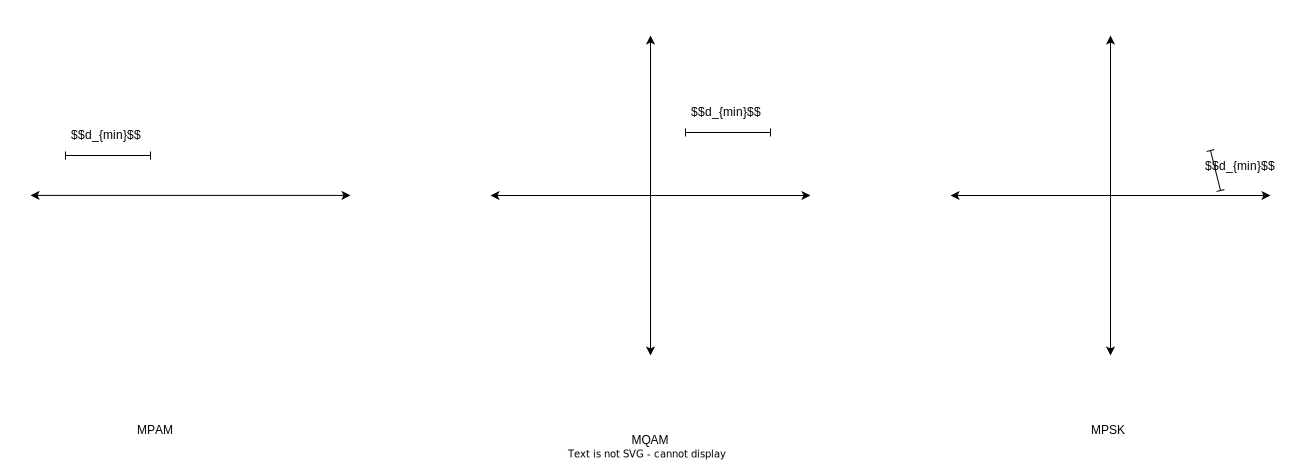
\includegraphics[width=0.75\textwidth]{figs/constellations.pdf}
  \caption{Constellation schemes where Quadrature and In-Phase possible discrete options are displayed in terms of their energy.}
  \label{fig:constellations}
\end{figure*}

\begin{table}[htbp]
  \centering
  \caption{}
  \begin{tabular}{lcccc}                                                                                                                   \\
    \cmidrule(r){1-5}  & MPAM                           & MPSK                       & MQAM                         & FSK     \\
    \midrule $E_s$     & $\frac{d_{min}^2}{12}(M^2-1)$  & $d^2$                      & $\frac{d_{min}^2}{6}(M^2-1)$ & $d^2/2$ \\
    \midrule $d_{min}$ & $\sqrt{\frac{12E_s}{M^2 - 1}}$
                       & $\sqrt{E_s}$                   & $\sqrt{\frac{6}{M^2 - 1}}$ & $\sqrt{2 E_s}$                         \\

    \bottomrule
  \end{tabular}
  \label{tab:win-space-results}
\end{table}


\section{Signal-to-noise ratio}


If the complex noise $n(t) \sim \mathcal{C}\mathcal{N}(0,2\sigma^2)$, meaning
each of the two channels is distributed as a zero-mean \gls{GRV} with variance
$\sigma$, this relates to the noise \gls{PSD} $N_0$ (in watts per hertz $W/Hz$)
as $\sigma^2 = N_0/2$. If the energy per dimension is $\bar{E_s} = E_s/2$, then
the \gls{SNR} is defined as:


\begin{align}
  \gamma_s = SNR = \frac{\bar{E_s}}{\sigma} = \frac{E_s}{2\sigma} = \frac{E_s}{N_0}
\end{align}

\Gls{SNR} can also be defined in terms of the power of the received signal $P_s$
over the power of the noise $P_n = N_0 B$, where $B = 1/T$ is the \gls{BW} of
the receiver. Note, the received signal power $P_s$ relates to the energy per
symbol as $P_s = E_s/T$ for a symbol time T.

\begin{align}
  \gamma_s = SNR = \frac{P_s}{P_n}= \frac{E_s/T}{N_0 B} = \frac{E_s}{N_0}
\end{align}


The \gls{SNR} also has an equivalent metric, the per-bit \gls{SNR} $Ebb-N_0$
expressed in terms of the energy per bit $E_b$ over the noise \gls{PSD} $N_0$.
The energy per bit is $E_b = E_s/\log _{2} M$. Also, define the bit-rate as $R =
  \frac{\log _{2} M}{T}$.

\begin{align}
  \gamma_b = Ebb-N_0 = \frac{E_b}{N_0} = \frac{ E_s/\log _{2} M}{N_0} = \frac{\gamma_s}{\log _{2} M} = \gamma_s \frac{B}{R}
\end{align}

\section{Probability of Error for fixed SNR}
TODO

The probability of error $P_s$ is defined in a per-symbol basis. Each constellation has a different $P_s$, seen in the table below based on the Nearest Neighbor bound in an \gls{AWGN} channel.

\begin{table}[htbp]
  \centering
  \caption{}
  \begin{tabular}{lcccc}                                                                                                                                            \\
    \cmidrule(r){1-3} & $P_s(\gamma_s)$                                  & $P_b(\gamma_b)$                                                             \\
    \midrule MPAM     & $2(1-1/M)Q(\sqrt{\frac{6\gamma_s}{M^2-1}})$      & $\frac{2(1-1/M)}{\log_{2}M}Q(\sqrt{\frac{6\gamma_b\log_{2}M}{M^2-1}})$      \\
    \midrule MPSQ     & $2Q(\sqrt{2\gamma_s}\sin(\pi/M))$                & $\frac{2}{\log_{2}M}Q(\sqrt{2\gamma_b\log_{2}M}\sin(\pi/M))$                \\
    \midrule MQAM     & $4(1-1/\sqrt{M})Q(\sqrt{\frac{3\gamma_s}{M-1}})$ & $\frac{4(1-1/\sqrt{M})}{\log_{2}M}Q(\sqrt{\frac{3\gamma_b\log_{2}M}{M-1}})$ \\
    \midrule FSK      & $(M-1)Q(\sqrt{\gamma_s/2})$                      & $\frac{(M-1)}{\log_{2} M}Q(\sqrt{\gamma_b \log_{2} M/2})$                   \\
    \bottomrule
  \end{tabular}
  \label{tab:constellation_pe}
\end{table}

Where generally $P_b = P_s / \log{2}(M)$ for Gray coded constellations.

Useful approximations for $0 \leq \gamma_s \leq 30$ dB:
\begin{itemize}
  \item MQAM $M \geq 4$ has $P_b(\gamma_s) \approxeq 0.2 e^{\frac{-1.5\gamma_s}{M-1}}$
  \item BPSK has $P_b(\gamma_s) = P_s(\gamma_s) \approxeq 2 e^{-1.5\gamma_s}$
\end{itemize}

Another way to more easily calculate

\section{Probability of Error for stochastic SNR}
Since the SNR depends on the received power, which in turn depends on the
affects of blocking, shadowing, and fading, the SNR is a random variable. It
becomes useful then to define the average \gls{BER}.

\begin{align}
  \overline{P_b}  \triangleq \E{P_b} = \int_0^{\infty} P_{b}(\gamma) f_{\gamma}(\gamma) d\gamma
\end{align}
\begin{mdframed}

  \subsection*{Average BPSK in Rayleigh Fading}
  Express the average \gls{BER} of a BPSK signal in a Rayleigh fading channel in terms of the averge SNR $\overline{\gamma}$.
  \\
  \\
  Answer: \\
  For Rayleigh fading:
  \begin{align}
    f_{\gamma_s}(\gamma) = \frac{1}{\overline{\gamma}} e^{-\gamma/\overline{\gamma}}\nonumber
  \end{align}
  And for BPSK:
  \begin{align}
    P_b(\gamma_s) = 2Q(\sqrt{2\gamma_s}) \nonumber
  \end{align}

  So the \gls{BER} is:
  \begin{align}
    \overline{P_b} & = \int_0^{\infty} 2Q(\sqrt{2\gamma}) \frac{1}{\overline{\gamma}} e^{-\gamma/\overline{\gamma}} d\gamma \nonumber
  \end{align}
  with change of variables $x = \gamma/\overline{\gamma}$ such that $d \gamma/\overline{\gamma} = d x $

  \begin{align}
    \overline{P_b} & = \int_0^{\infty} 2Q(\sqrt{2x\overline{\gamma}}) e^{-x} dx \nonumber                                         \\
                   & = \frac{2}{2\pi} \int_0^{\infty} e^{-x} \int_{\sqrt{2x\overline{\gamma}}}^{\infty} e^{-t^2/2} dtdx \nonumber
  \end{align}
  and switching the order of the integrals
  \begin{align}
    \overline{P_b} & = \frac{1}{\pi} \int_0^{\infty} \int_{0}^{t^2/(2\overline{\gamma})} e^{-t^2/2} e^{-x}  dxdt \nonumber \\
                   & = \frac{1}{\pi} \int_0^{\infty} e^{-t^2/2}(1-e^{t^2/(2\overline{\gamma})}) dt \nonumber               \\
                   & = \frac{1}{2} - \frac{1}{1\pi} \int_0^{\infty} e^{-t^2(1+1/\overline{\gamma})/2} dt \nonumber         \\
                   & = \frac{1}{2} \left( 1-\sqrt{\frac{\overline{\gamma}}{1+\overline{\gamma}}}\right) \nonumber          \\
                   & \approxeq \frac{1}{4\overline{\gamma}} \nonumber
  \end{align}
\end{mdframed}

As seen in the example above it can become cumbersome to calculate the average
bit error rate. To expedite the process we can use the moment generating
functions of the channels and simplify the integral. Most constellation bit
error probabilities can be approximated or precisely expressed as $$P_b(\gamma)
  = a Q( \sqrt{\beta\gamma})$$

Using \cite{Craig258319}, we can express the $Q$-function as
\begin{align}
  Q(x) = \frac{1}{\pi}\int_{0}^{\pi/2} e^{-\frac{x^2}{2 \sin^2\phi}}d\phi
\end{align}
TODO

\chapter{Diversity}


\chapter{Channel Capacity}

\section{AWGN Channel Capacity, no fading}
The capacity of a channel is a measure of the amount of information that can be
transmitted over the channel, and is denoted with $C$. Another representation is
with channel efficiency where the capacity is divided by the signal \gls{BW}
denoted with B.

\begin{align}
  C   & = B log_{2}(1+\gamma) ~~ bps/ \text{complex channel}           \\
  C/B & = log_{2}(1+\gamma) ~~ bps/Hz/ \text{complex channel\nonumber}
\end{align}

\begin{mdframed}

  \subsection*{Shannon Capacity/ \gls{AWGN} Capacity derivation}
  Derive the Shannon capacity using mutual information.
  \\
  \\
  Answer: If an \gls{AWGN} channel $y = x + w$ where $w \sim \mathcal{N}(0,N_0)$
  then the capacity is equal to the maximum amount of mutual information
  $I(x,y)$ of the channel input and output.
  \begin{align}
    C/B & = \max_{x} I(x;y) = \max_{x} \left[h(y) - h(y|x) \right] \nonumber \\
        & = \max_{x} \left[h(x+w) - h(x+w|x) \right] \nonumber               \\
        & = \max_{x} \left[h(x+w) - h(w) \right] \nonumber
  \end{align}

  For a \gls{GRV} $w$, the entropy $h(w) = \frac{1}{2} \log_{2} (2 \pi e N_0)$.
  Also, the distribution which maximizes differential entropy $h$ for random
  variables of the same variance is Gaussian. This means maximizing $C$ can be
  boiled down to maximizing $h(x+w)$, which happens when $x+w \sim
    \mathcal{N}(\mu,\sigma^2)$. This is true only when $x \sim
    \mathcal{N}(0,P_x)$.
  \begin{align}
    \therefore C/B & = \max_{x} I(x;y) = \frac{1}{2} \log_{2}(2\pi e (E_s + N_0)) - \frac{1}{2} \log_{2} (2 \pi e N_0) \nonumber \\
                   & = \frac{1}{2} \log_{2}(1 + \frac{E_s}{N_0}) = \frac{1}{2} \log_{2}(1 + \gamma)
  \end{align}
  For $x$ a complex \gls{GRV} the capacity is doubled.
\end{mdframed}

\section{Flat Fading Channel Capacity}
In this regime, the \gls{SNR} of the channel is a \gls{rv} due to fading. Since the noise is always modeled as Gaussian, what we model making the  \gls{SNR} of a channel a  \gls{rv} is the time-varying gain of a channel. The instantaneous received \gls{SNR} at time $i$ is a function of the average transmit power $\overline{P_x}$, the noise \gls{PSD}, signal \gls{BW} and instantaneous gain of the channel at time $i$ $g[i]$.

The capacity of the channel, then, depends on the knowledge of the channel gain, called the \gls{CSI}. There are three choices regarding the \gls{CSI}:

\begin{itemize}
  \item \gls{CDI}: Both transmitter and receiver known the distribution of $g[i]$
  \item Receiver \gls{CSI}: Only the receiver knows the value of $g[i]$, but both transmitter and receiver known the distribution of $g[i]$
  \item Receiver \& transmitter \gls{CSI}:  Both transmitter and receiver known the distribution and the value of $g[i]$
\end{itemize}

\subsection{Channel Distribution Information}
CDI is an open problem. It can become difficult to find the capacity-achieving
distribution for the input. Literature exists on specific cases, such as the
Rayleigh fading channel, in which the power gain is exponentially distrubuted
and changes with each channel use at time $i$. An optimal solution exists, but
the optimal distribution and capacity must be found numerically and lacks a
closed-form solution.
TODO
\subsection{Receiver Channel Side Information}
In this case the capacity is defined by the Shannon capacity. In practical systems the rate cannot be maintained constant as is expected in Shannon capacity, so a reduction from the Shannon capacity is expected.

Shannon (ergodic) capacity can be computed by integrating over the distribution of the \gls{SNR}, which is known by both the transmitter and receiver.

\begin{align}
  C & = \E{B\log_{2}(1+\gamma)} =\int_0^{\infty}B \log_{2}(1+\gamma)p(\gamma)d\gamma
\end{align}

Since the realization of $\gamma$ is known only to the receiver, the ergotic capacity is constant, regardless of $\gamma$. A bound on the capacity can be roughly formed by using Jensen's inequality and switching the expectation and logarithm to achieve
\begin{align}
  C & \leq B\log_{2}(1+\E{\gamma}) = B\log_{2}(1+\overline{\gamma})
\end{align}
where $\overline{\gamma}$ is the average channel \gls{SNR}. This shows that for receiver \gls{CSI}, the achievable capacity is always less than the Shannon capacity.

\subsection{Receiver \& Transmitter Channel Side Information}
In this regime, the receiver can feed back information about the channel to the transmitter, and in turn the transmitter can take actions and adapt it's transmission strategy.

There are two main knobs which the transmitter has access to in order to change it's strategy: power and rate. If we allow the transmit power to vary with some function of $\gamma$ subject to some average power constraint $\overline{P}$, we arrive at the power adaptation strategy.

\subsection*{Water filling: Optimal Strategy}
TODO
Solving the resulting lagrangian from
\begin{align}
  C = \max_{P(\gamma)} \left[ \int_{0}^{\infty}B \log_2 (1 + \frac{P(\gamma)}{\overline{P}}\gamma)p(\gamma) d\gamma\right] \nonumber \\
  \text{s.t. } \int P(\gamma)p(\gamma)d\gamma = \overline{P}
\end{align}

results in a \gls{WF} solution where
\begin{align} \label{PA_policy}
  \frac{P(\gamma)}{\overline{P}} = \left\{ \begin{array}{ll}
                                             1/\gamma_0 - 1/\gamma & \gamma \geq \gamma_0 \\
                                             0                     & \gamma < \gamma_0    \\
                                           \end{array}
  \right.
\end{align}

for the value of $\gamma_0$ that satisfies the power constraint from the lagrangian. The overall capacity in the receiver and transmitter \gls{CSI} is then:
\begin{align}
  C = \int_{\gamma_0}^{\infty} B \log_{2} (\frac{\gamma}{\gamma_0})p(\gamma)d\gamma
\end{align}

Since the power adaptation policy in (\ref{PA_policy}) has a dependence on the threshold, it can only be achieved with a time-varying data rate achieved for the instantaneous \gls{SNR}. For Rayleigh fading, this capacity can exceed the AWGN channel capacity for the same average SNR, different to the \gls{CSI} case where fading always indicated decreased capacity.

For an arbitrary power adaptation policy, the channel capacity is
\begin{align}
  C = \int_{\gamma_0}^{\infty} B \log_{2} (1 + \frac{P(\gamma)}{\overline{P}}\gamma)p(\gamma)d\gamma
\end{align}

\subsection*{Discrete Rate adaptation}
Since the \gls{WF} is not practically achievable, a discrete Rate adaptation method is described where the transmitter can choose the rate between discrete scemes (i.e. MQAM with varying M).
TODO
\subsection*{Power Adaptation at fixed rate}
The power adaptation scheme employed here is:
\begin{align} \label{PA_policy_fixedR}
  \frac{P(\gamma)}{\overline{P}} = \left\{ \begin{array}{ll}
                                             \gamma_t/\gamma & \gamma \geq \gamma_0 \\
                                             0               & \gamma < \gamma_0    \\
                                           \end{array}
  \right.
\end{align}
for some target \gls{SNR} $\gamma_t$.
\printglossary[type=\acronymtype,title=Acronyms]

\bibliographystyle{ieeetran}
\bibliography{ref}
\end{document}

